\chapter*{Conclusion et perspectives}
\markboth{\MakeUppercase{Conclusion et perspectives}}{\MakeUppercase{Conclusion et perspectives}}
\addcontentsline{toc}{chapter}{Conclusion et perspectives}
\setcounter{figure}{0}

Les différents travaux réalisés durant ma thèse ne sont que les premières étapes dans le développement d'une véritable spintronique à l'échelle de la molécule unique. Ils ont cependant révélé de nombreux aspects très prometteur quant à l'utilisation de l'interaction entre le transport électronique et le magnétisme moléculaire. En effet, grâce à la réalisation d'un transistor à molécule unique basé sur l'utilisation d'un aimant moléculaire (Fig 1.a), la faisabilité d'une électronique moléculaire pour laquelle le magnétisme à l'échelle d'un moment magnétique unique peut être sondé a été démontré. 

En effet, nous avons tout d'abord montré que la conductance de notre transistor était dépendante de l'orientation du moment magnétique d'une molécule unique. Correctement utilisée, cette propriété nous a tout d'abord permis d'observer le retournement de l'aimantation par effet tunnel à l'échelle d'un moment unique. Cette capacité de mesure fait également, de notre technique, un détecteur d'une très grande sensibilité qui pourrait être utilisé dans le cadre du magnétisme moléculaire pour l'investigation des propriétés quantiques des aimants moleculaires à l'échelle de la molécule unique. Ainsi, la méthode que nous avons développée afin de reconstituer le cycle d'aimantation à l'échelle d'une molécule unique pourrait contribuer à cette étude (Fig1.b). Cette mesure montre clairement les différences qu'il existe entre une mesure effectuée sur une assemblée par rapport à une molécule unique, dans le cas de l'aimant moléculaire TbPc2. Dans notre cas, à faible champ magnétique, uniquement les quatre marches préditent théoriquement sont visibles. Dans le cas d'une assemblée, une multitude de marche supplémentaire ont été observées, montrant clairement l'influence de l'environnement moléculaire de la moléculaire sur son comportement magnétique.

Figure 1
Fig1.a : image Mario
Fig1.b : image hystérésis

De plus, dans le cas de cet aimant moléculaire, grâce à la corrélation intrinsèque qu'il existe entre le moment magnétique et l'état de spin nucléaire, nous sommes parvenus à réaliser une mesure électrique d'un spin nucléaire unique. Cette réalisation, portant la sensibilité magnétique de notre technique de mesure à quelques millièmes de muB, s'est également avérée non destructive de l'état du spin nucléaire. Nous avons ainsi étudié la dynamique d'un spin nucléaire unique. Un long temps de vie de l'état d'un spin de l'ordre de 10 secondes a tout d'abord été mesuré, alors que sa température était proche de la température électronique de notre réfrigérateur à dilution. Ces différents résultats ouvrent donc la voie expérimentale à la proposition théorique de Kane [ref] relatant de l'utilisation d'un spin nucléaire unique comme base d'une électronique de spin.


Cependant, différents points restent encore mystérieux dans les différentes mesures que j'ai présentées. En effet, une étude de la relaxation que nous avons menée pour deux points de fonctionnement bien différents montre clairement que la dynamique du spin nucléaire est fortement dépendante de l'environnement électrostatique, et donc, du régime de transport. Si le ou les mécanismes régissant cette dependance ne sont pas encore identifiés. Ils conduisent pourtant a une modification importante du temps de vie  (cf Chap. 3), mais également à des transitions supplémentaires mesurées lorsque l'on se situe à gauche (état de charge pair) ou à droite (état de charge impair) du point de dégénérescence de charge nous servant de sonde(cf Fig.3.1.c). Ainsi, une étude plus approfondie doit encore être menée afin de comprendre les mécanismes responsables de cette dépendance.
En effet, il apparaît primordial de démontrer si ces différents phénomènes ne sont que la manifestation d'un seul et même mécanisme. De manière plus générale, une compréhension accrue des phénomènes de couplage entre le magnétisme moléculaire et son environnement nous parait indispensable.

Dans le cadre des transitions supplémentaires observées sous certaines conditions, si certaines ont été identifiées comme provenant de l'environnement moléculaire de la molécule étudiée, nous avons également mesuré un autre type de transition dont le position est dépendante du champ transverse appliquée.

Fig2 : drapeau anglais sans les transissions flip-flop.

Cette mesure présente deux types de transitions : les transitions correspondantes aux événements de retournement de l'aimantation par effet tunnel de la molécule étudiée, mais également un jeu de 4 transitions évoluant avec le champ transverse, que nous nommerons pas la suite transition induite. Une direction afin de comprendre et d'expliquer ces transitions induites semblent être le couplage du terbium avec un autre point quantique dans l'environnement de la molécule, mais ne participant pas au transport. Si cette première étude de ces transitions induites (cf Fig.3.1.b) nous permet de penser que ces dernières sont dues a l'interaction entre la molécule aimant et un second système magnétique, la nature de ce système magnétique et de l'interaction qui le couple a l'aimant moléculaire restent encore à déterminer. Le travail des théoriciens a ce sujet nous apparaît indispensable à l'analyse, mais également à la poursuite des mesures.



Cependant, de nombreux aspects de nos travaux peuvent encore être améliorés. La fabrication de nos échantillons tout d'abord qui, à ce stade, n'exploite pas encore les possibilités offertes par l'approche ``Bottom-Up" évoquée dans le premier chapitre. En collaboration avec notre groupe, Sébastien Liatard, dans le cadre de sa thèse, a mené une étude préliminaire allant dans cette direction. La technique sur laquelle il travaillait consistait à venir attacher une molécule, par des moyens chimiques, à deux billes d'or (cf Fig.3.1.a). Il faisait ensuite, à partir de ces billes, croître des bâtonnets d'or de plusieurs centaines de nanomètre de longueur qu'il serait ensuite facile de contacter. Ces travaux n'ont malheureusement pas pu être menés à leur terme, et n'ont donc pas conduit à la fabrication d'un dispositif fonctionnel. Il nous apparaît donc nécessaire de poursuivre dans cette voie afin d'obtenir des dispositifs en plus grand nombre et de manière reproductible. On peut imaginer une mémoire entièrement constituée de jonctions moléculaires, permettant de disposer d'une grande densité de stockage.




Petite intro sur la manipulation de spin dans les aimants moléculaires [ref des oscillations de Rabi sur Fe4 avec l'image] pour très rapidement dire qu'il y a mieux, i.e. :



Enfin, la manipulation et la lecture des etats du spin nucléaire est une étape essentielle vers la réalisation d'un qbit à base de molécules aimants. Si nous avons démontre comment réaliser l’étape de lecture, reste encore à mettre en œuvre l’étape de manipulation. On pourrait pour cela profiter de l'espacement inégal des énergies des différents états de spin, pour implémenter un schéma de pompe/sonde comme présenté dans la Fig.3.1.d. Une première étape consistant en un pulse d'une fréquence $\nu_1$ initialiserait le spin nucléaire de l’état $|0\rangle$ à l'etat $|1\rangle$. Un temps variable séparerait cette étape d'un second pulse de fréquence $\nu_2$ permettant la transition de l’état $|1\rangle$ à l’état $|2\rangle$. La lecture se ferait ensuite par le procédure que l'on a présentée dans le Chap.3. On pourrait ainsi mettre en évidence des oscillations de Rabbi par des mesures en transport, accédant au $T_2$ du spin nucléaire, et réaliser le premier qbit à base d'aimant moléculaire.

Fig

Du fait de la répartition anharmonique des niveaux d’énergies du spin nucléaire, une procédure plus complexe pourrait également être développée mettant en jeux un nombre plus élevé de pulses radio-fréquences (RF) dont la polarisation serait contrôlée. Une telle procédure permettrait d’implémenter l'algorithme de Grover, comme cela a été détaillé par Loss et al. dans [ref ! !].

\begin{figure}
\centering 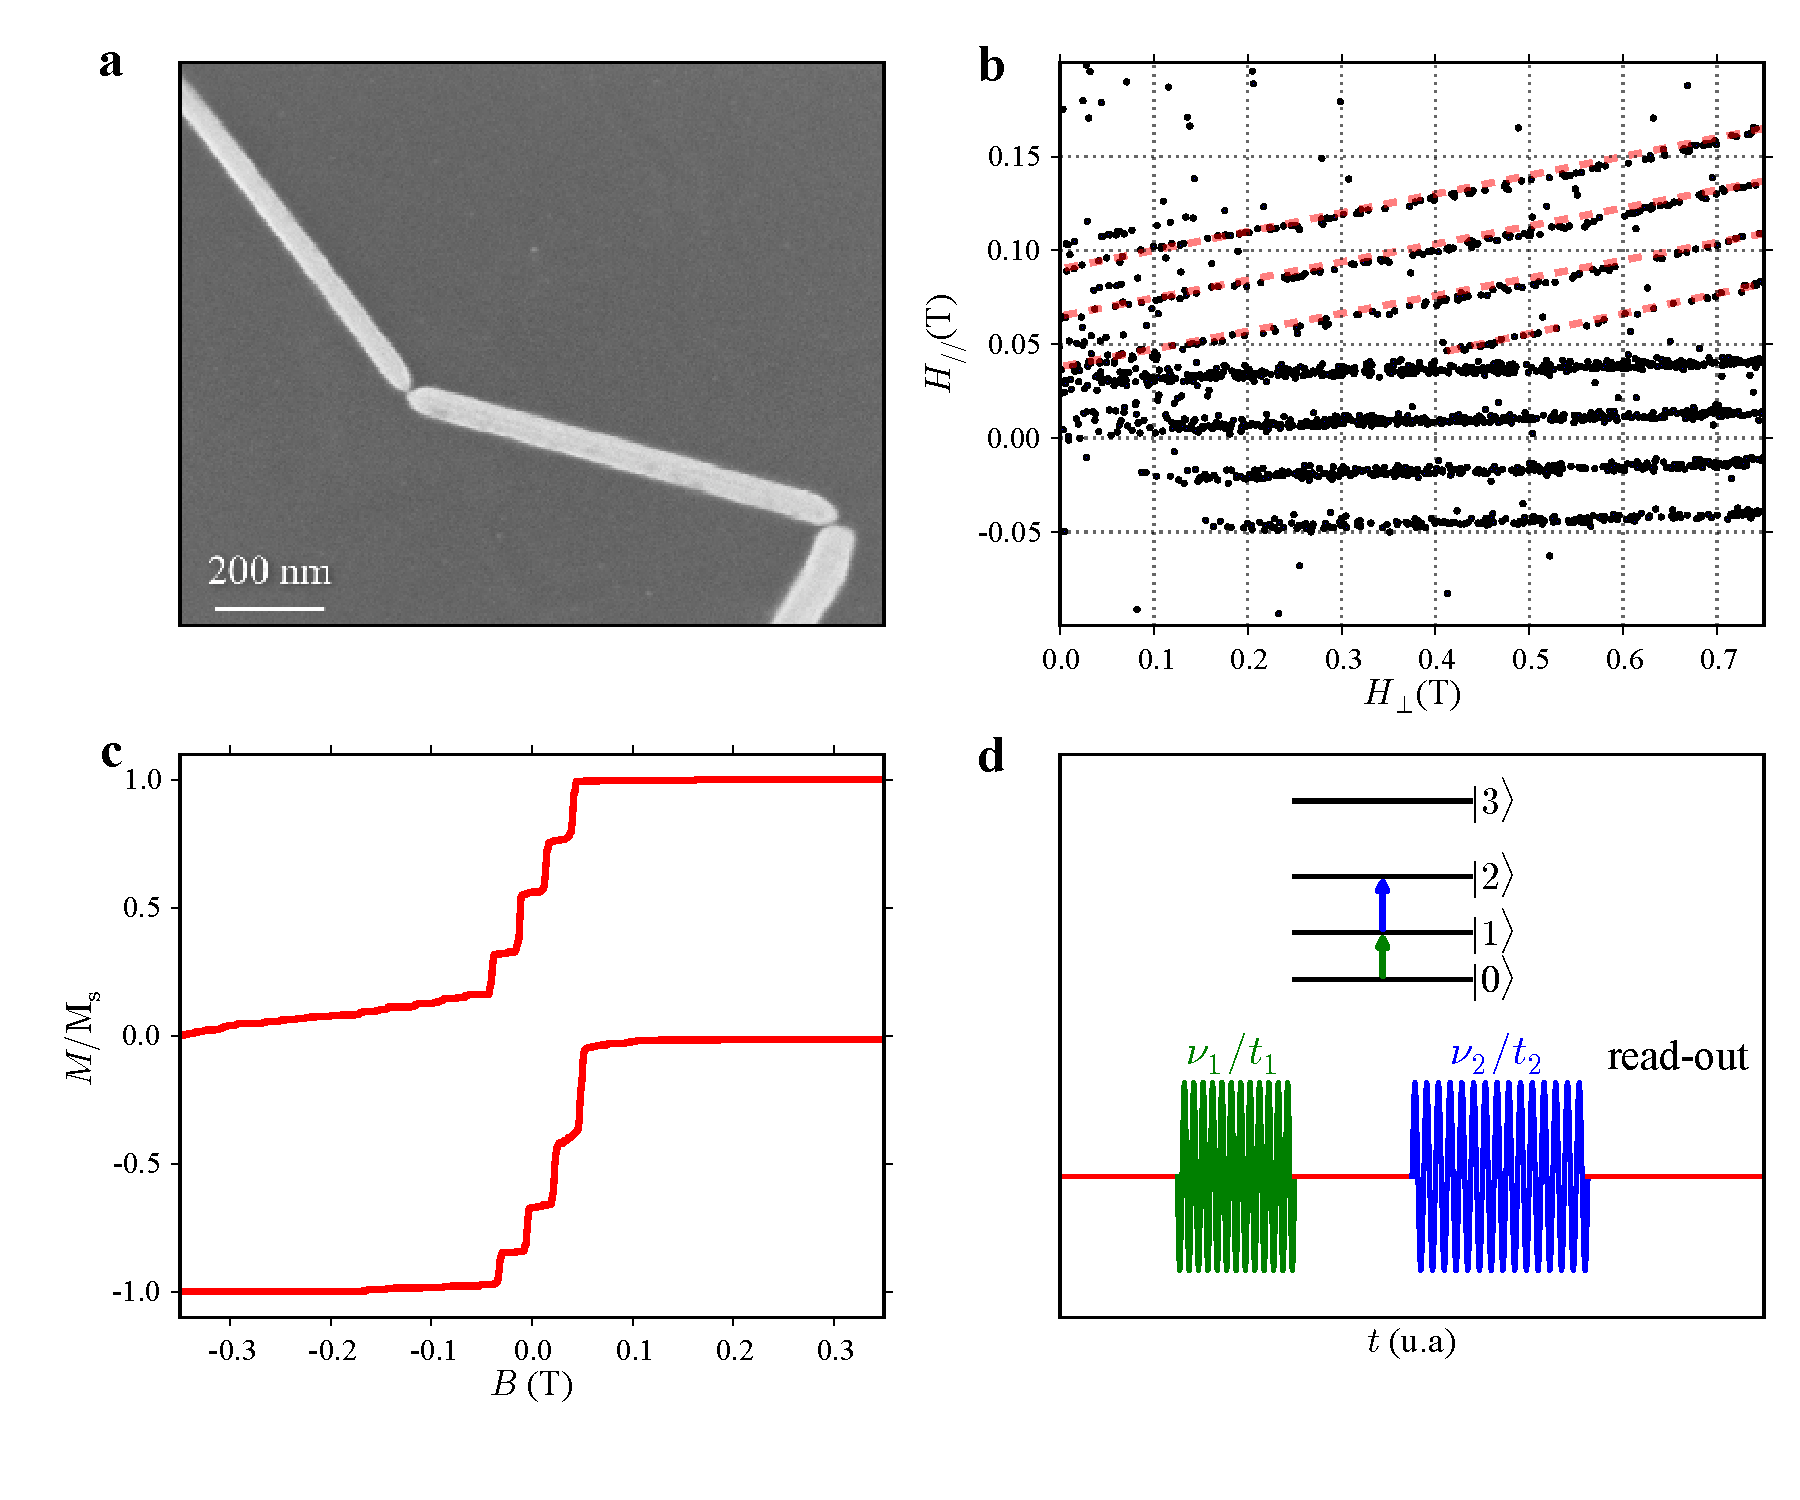
\includegraphics[scale=0.45]{Conclusion/Perspectives/Perspectives.pdf} 
\caption{\textbf{a} : deux bâtonnets d'or obtenus à partir de la croissance de deux billes d'or reliées entre-elles par des molécules~(extrait de [thèse de Sebastien]). \textbf{b} : étude de la position des transitions induite en fonction du champ parallèle et du champ transverse. Chaque point marque un retournement de l'aimantation. Les transitions surligné en rose corresponde à des renversements induits par le couplage de l'aimant moléculaire avec un seconde système magnétique. \textbf{c} : reconstruction du cycle d'hystérésis obtenu en régime Kondo. Seules les transitions correspondantes au phénomène de QTM sont visible. \textbf{d} : schéma de la technique de pompe-sonde. Une première fréquence $\nu_1$ initialise l'état de $|0\rangle$ à l'état $|1\rangle$. Puis un second pulse fait passer le système de l'état $|1\rangle$ à m'état $|2\rangle$. On effectue ensuite la lecture de l'état par la méthode présentée au Chap.3.}
\label{Perspectives}
\end{figure}

